\section{Related Work and Discussion}
\label{sec:discussion}





As mentioned earlier, there are many recent and ongoing efforts to prototype disaggregated hardware. We discussed the salient features of these efforts inline throughout this paper and hence we only briefly elaborate on them here. 

Lim \etal~\cite{ddcHwDesign1, ddcHwDesign2} discuss the trend of growing peak compute-to-memory ratio, warning of the ``memory capacity wall'' and prototype a disaggregated memory blade. Their results demonstrate that memory disaggregation is feasible and can even provide a 10x performance improvement in memory constrained environments. As noted earlier, our study focuses on the (for us) worst-case scenario where applications are not memory constrained in the non-disaggregated scenario and hence the potential performance degradation due to disaggregation is high. For the same reason, we did not consider redesigning applications to exploit the plentiful remote memory available in \dis. 

Sudan \etal~\cite{ddcHwDesign3} use an ASIC based interconnect fabric to build a virtualized I/O system for better resource sharing. However, these interconnects are designed for their specific context; the authors neither discuss network support for disaggregation more broadly nor consider the possibility of leveraging known datacenter network technologies to enable disaggregation.

Firebox~\cite{firebox} proposes a holistic architecture redesign of datacenter racks to include $1$Tbps silicon phonics links, high-radix switches, remote nonvolatile memory, and System-on-Chips (SoCs). Theia~\cite{theia} proposes a new network topology that interconnects SoCs at high density. Huawei's DC3.0 (NUWA) system uses a proprietary PCIe-based interconnect. R2C2~\cite{r2c2} proposes new topologies, routing and congestion control designs for rack-scale disaggregation.
None of these efforts evaluate network requirements based on existing workloads as we do, nor do they evaluate the effectiveness of existing network designs in supporting disaggregation, or the possibility of disaggregating at scale.

%Overall, we find that related work confirms our prediction that sub-$5\mu$s latencies are feasible in the near future. 

In an early position paper, Han \etal~\cite{hotnets} measure -- as we do -- the impact of remote memory access latency on application-level performance within a single machine. Our work extends this  understanding to a larger set of workloads and concludes with more stringent requirements on latency and bandwidth than Han {\it et al} do, due to our consideration of shark applications. In addition, we use simulation and emulation to study the impact of queueing delay and transport designs which further raises the bar on our target network performance.

%understanding along the new network-oriented design parameters of latency, bandwidth, and transport.Furthermore, our evaluation includes evaluation of additional applications and runs on a cluster of machines ``in the wild,'' measuring realistic scenarios which may have been hidden in a single-machine setting. 

%\paragraphb{Low Latency}
Multiple recent efforts~\cite{farm,mica,herd,ramcloud} aim to reduce the latency in networked applications through techniques that bypass the kernel networking stack, and so forth. %for significant latency improvements with Infiniband RDMA and direct NIC access. 
%Looking forward, CPU-NIC integration, in which the OS kernel and device driver are more directly involved in the low-level operation of the NIC, is on the Simia
Similarly efforts toward NIC integration by CPU architects~\cite{cpu-nic} promise to enable even further latency-saving optimizations. As we note in \S\ref{ssec:rtt}, such efforts are crucial enablers in meeting our latency targets. 

\cut{ 
\paragraphb{Specialized Hardware}
While these innovative hardware technologies may unlock future gains in application performance and capabilities, they are complementary rather than necessary for disaggregation.

\paragraphb{Shared Pool Abstraction}
Managing large pools of compute resources will be a challenge for disaggregated datacenters. In this vein cluster managers such as Mesos~\cite{mesos} and resource schedulers such as DRF~\cite{drf} may prove useful in efficiently allocating resources to applications.

\paragraphb{Networks in Disaggregated Datacenters}
R2C2~\cite{r2c2} explores the problem of designing a network stack for rack-scale computers, proposing an interconnect topology for disaggregation at the rack-scale and explore the questions of designing efficient routing and congestion control mechanisms in the context of rack-scale disaggregation.
Our study finds that such efforts at enabling disaggregation at the rack scale with specialized interconnects and protocols \an{are largely unnecessary to achieve application performance.}
} 








\begin{figure}
  \centering
    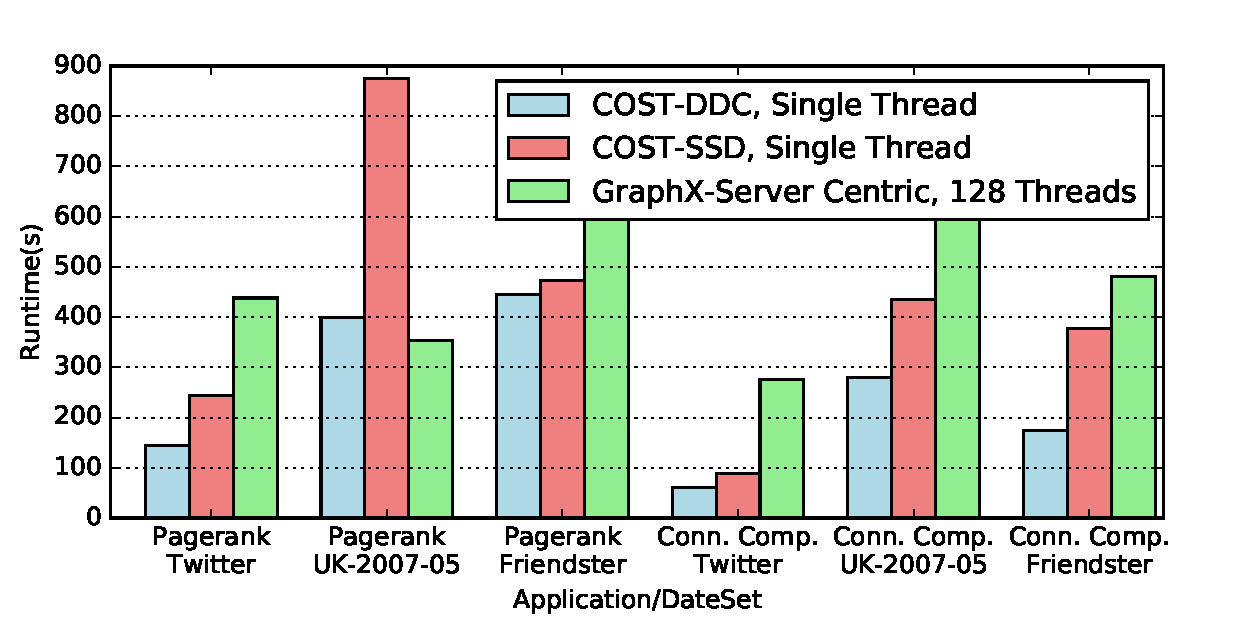
\includegraphics[width = \columnwidth]{img/benefit.eps} 
  \caption{\small{Running COST in a simulated DDC. COST-DDC is 1.48 to 3.04 faster than GraphX-Server Centric. The datasets we evaluated are, Twitter (4.17m nodes, 1.47b edges), UK-2007-05 (105m nodes, 3.7b edges), and Friendster (65m nodes, 1.8b edges)}}
  \label{fig:benefit}
\end{figure}


\subsection{Improve App Performance in DDC}
While most of the existing applications' performance does not degrade significantly in a DDC, we envision that applications could be rewritten to fully take advantage of disaggregation. 
A recent paper from McSherry et. al.~\cite{cost} shows that current server centric architecture incurs high overhead to scale out.
For applications such as distributed graph engines, the coordination and communication overhead is too substantial for them to benefit from parallelism.

We conduct a similar experiment as COST~\cite{cost} to show that applications adapted to disaggregated environment can outperform traditional server centric ones.
To simulate an application running in a DDC, we setup a virtual machine with 4 cores and 3GB of memory. 
The server is capable of accessing an ``infinitely'' large remote memory pool by swapping to a RDMA-backed block device. 
We run Pagerank and Connected Components using COST, a single thread graph compute engine over three large graph datasets.
Since COST mmaps the input file, we store the input files into another RDMA-backed block device.
For server centric architecture, we evaluate GraphX using a 16-node m2.4xlarge cluster on EC2. 
Figure \ref{fig:benefit} shows the application runtime of COST-DDC and GraphX-Server Centric.
For most of the case, COST-DDC is 1.48 to 3.04 times faster than GraphX-Server Centric, except Pagerank on UK-2007-5 dataset. 
After talking to one of the author of GraphX, we discovered that the UK-2007-05 dataset has better partition property such that there are fewer vertices spanning machines, hence GraphX performs well. 
We also evaluate the performance benefit of using remote memory over local SSD.
From Figure ~\ref{fig:benefit}, swapping using RDMA is 1.06 to 2.15 times faster than its SSD counterpart. 













\cut{
\paragraphb{Research prototypes} \rc{Remove? Already discussed in S2 $\to$} Rack-scale disaggregation has been attracting a lot of attention recently, both in industry and in academia. Early industry rack scale prototypes include AMD SeaMicro~\cite{seamicro}, Intel RSA~\cite{rsa}, HP's The Machine~\cite{hptm}, and Facebook's Disaggregated Rack~\cite{fdr}. Indeed, several of the assumptions that led to our observations were motivated by these designs. For instance, the architecture in HP's The Machine closely resembles the hardware and software architecture in \S\ref{sec:summary} --- CPU blades with small local cache connected to four massive pools of memory via network-wide interconnect (optical, in this case). Indeed, each CPU blade uses $256$GB of local cache, while the memory blades have 1TB of main memory.

There are several other research prototypes such as soNUMA~\cite{sonuma}, Catapult~\cite{catapult}, and Firebox~\cite{firebox}.
Firebox~\cite{firebox}, for example, is a disaggregated prototype using high-radix silicon photonic switches to connect SoCs and memory modules numbering in the thousands.

While our study was motivated by above trends, we focused on the network requirements from resource disaggregation, a problem that has not been explored by any previous work. We believe such a study will not only impact the design of networks for disaggregated datacenters, but may also shed light on how constraints from the network may impact future proposals on resource disaggregation.

\rc{The following text needs to be modified based on the story; put our work in context of the related work $\to$}

% These projects do not focus on the network design questions that we address; our efforts are complementary and may be useful in informing the design of such systems.

%It's not us! see, we're referring to ourselves in the third person yay double blind science
Han \etal~\cite{hotnets} focused on understanding the impact of remote memory access latency on application-level performance within a single machine. This work extends this understanding along the new network-oriented design parameters of latency, bandwidth, and transport.
Furthermore, our evaluation includes more applications and runs on a cluster of machines ``in the wild,'' measuring realistic scenarios which may have been hidden in a single-machine setting. 

%First, our evaluation on understanding the impact of remote data accesses runs in the wild, capturing realistic scenarios which may otherwise be hidden on a single-machine setting. Our work also extends~\cite{hotnets} by characterizing the network traffic in disaggregated datacenters, and exploring how the new traffic patterns may impact the application-level performance using existing network designs. 
\paragraphb{Disaggregated Datacenter Designs}
Existing prototypes and efforts in disaggregated datacenters~\cite{hptm, rsa,fdr,firebox,seamicro,catapult}, as discussed in \S\ref{ssec:prototype}, differ from our work in that their assumed scope of disaggregation is rack scale and they use specialized network designs inside their rack scale systems. 

%\paragraphb{Specialized hardware for disaggregation}

\paragraphb{Distributed Shared Memory (DSM)}
There has been much recent activity in implementing distributed shared memory environments for big data analytics. FaRM~\cite{farm}, MICA~\cite{mica}, Herd~\cite{herd}, and Grappa~\cite{grappa} all employ RDMA to enable fast remote reads in distributed settings. These systems not only demonstrate the benefits of remote memory accesses, but also show that RDMA and new technologies may enable the low latency requirements outlined in our study. Our study can inform future efforts in building applications tuned for disaggregated datacenters.







% RDMA allows remote memory access without OS involvement and hence enables efficient memory sharing between servers in datacenter.
% FaRM~\cite{farm} does lock-free reads over RDMA and enables single machine transaction using function shipping. 
% Grappa~\cite{grappa} is a software distributed memory system for data-intensive applications.
% These systems demonstrate the benefits of memory sharing and show that RDMA could improve the efficiency of memory sharing.


%The focus of our study is orthogonal to that of R2C2. Rather than designing disaggregated datacenter networks, our study aims to build an understanding of network requirements, traffic characteristics, and sufficiency of existing network designs in the context of resource disaggregation. Our study may help building an understanding of these issues, and guide the design of network topologies and protocols for resource disaggregation. 

% R2C2~\cite{r2c2} designs a torus like topology to increase the path density in its rack scale network.
% By leveraging the relatively small scale of the network, R2C2 uses a broadcasting protocol to ensure all nodes in the network are aware of all the flows in the network.
% We believe broadcasting is cost prohibitive in datacenter scale distribution, and hence R2C2 is only suitable for rack scale disaggregation.





% \subsection{Limitations}
% One limitation of our results is our application-agnostic measurement approach. While this models disaggregation at the operating system level, it misses any potential application-specific considerations such as the interdependency of flows and its effect on performance. As a result we did not model potential application-specific optimizations such as custom data placement strategies or prioritizing flows based on the access dependency graph. We also did not study failure modes or running mixes of applications together. As a result our results focus on demonstrating the feasibility of disaggregation rather than showcasing novel designs. Future work in this regard may focus on improving resource packing or data access scheduling mechanisms.

\cut{ 

\sr{TBD: if we have time, let's consider adding the Spark results here presented as we went searching for a case where disaggregation fails. Found it in Spark. Explain why. And say that some apps will have to be rewritten. More generally, the question of what's the right  programming model is wide open.}
} 


%\subsection{Looking Ahead}

%In this section, we briefly discuss some of the research questions that disaggregation raises on three fronts: 
%i) approaches to building low-latency networks, ii) network architecture, and iii) systems architecture. Each of these merits a paper in itself; as such, what follows is more an enumeration than an in-depth discussion of potential issues.

%\subsubsection{Realizing Low Latency Networks}
%As demonstrated in \S\ref{sec:requirements}, building low latency networks (with round-trip times under of 10 us \rc{change number?}) will be critical for large scale disaggregation. 
%Fortunately, this is a topic of that has been receiving a great deal of attention in recent research and, coincidentally, a recent paper~\cite{lowlatency} argues the feasibility of such low latency in datacenter networks in the near future. 
%The authors cite the growing prevalence of cut-through switches and vendor plans for
%tighter integration of IO capabilities into the CPU as key enabling factors.
%In addition to the hardware trends, we believe there are many opportunities to further reduce network latency including improved protocol designs~\cite{pfabric, phost} and all-optical switches with no buffering. 
%The effectiveness and suitability of these approaches for disaggregation is a topic for future work.
%An orthogonal approach to reducing latency is to try and reduce the network distance between the resources allocated to a job, in much the same way that map-reduce schedulers today aim for data locality in scheduling tasks.
%Future research should study how to best distribute resource blades across racks and the design of scheduler optimizations for low latency.
%Finally, an important goal should be to achieve latencies that are not just low but also deterministic, since high variability will lead to unpredictable application performance. 
%An intriguing possibility here is the use of TDMA-based network architectures as proposed in recent work by Vattikonda et al~\cite{tdma}.


%\subsubsection{Network Architecture}

%We can probably build networks for disaggregated datacenters using existing networking technologies such as Ethernet, InfiniBand, or PCIe \rc{is this true????}. 
%An interesting research question - if only to understand what change might be desirable - is to ask what the ideal network architecture in support of disaggregation might look like.

%It is worth noting that disaggregation effectively blurs the lines between what used to be separate intra- and inter-server networks. E.g., in Figure \ref{fig:dc} we see that today’s server architecture includes networks for communication between CPUs (e.g., Intel QuickPatch Interconnect or AMD HyperTransport protocols), between CPUs and memory (DDR3) and to peripheral devices (e.g.,based on the PCIe protocol). 
%Traditionally, these intra- and inter-server technologies have evolved very differently. 
%Basic concepts such as variable-sized packets and best-effort service are common in inter-server networks but not so in intra-server links/networks. 
%The network in a disaggregated datacenter combines aspects of both; it is resource-centric (like intra-server networks today) but is less tightly integrated with the endpoints and must operate at scale (like existing inter-server networks) and hence picking new network abstractions should be done carefully.
%A starting point might be to ask whether packets are the right abstraction. Since both existing intra- (except for CPU-to-memory DDR3) and inter-server link protocols today use packet-like switched technologies, we believe packets remain the right abstraction. 
%An open question however is whether we would be better served with solutions that allow us to amortize per-packet processing overheads (for reduced latency) such as larger MTUs or a “packet bursts” abstraction. \rc{don't we address this? not really an open question...}
%A second question regards communication reliability. Clearly, the resource endpoints must see an end-to-end abstraction of reliable communication; however, it is not clear whether we need reliability at the level of individual network links (as found in intra-server link
%technologies and some inter-server links such as InfiniBand) or whether end-to-end retransmissions (as used with Ethernet networks) will suffice. 
%Our conjecture is that end-to-end retransmissions should be adequate given the low RTTs we envisage, however this is an important question that warrants more rigorous exploration.
%Another related question is whether we need support for bandwidth reservations, or fair resource sharing mechanisms, or whether pure statistical multiplexing with end-to-end congestion control will suffice. \rc{this is answered in section 5}
%There are many calls for reservations and fairness~\cite{faircloud,elasticswitch,seawall} even in existing datacenter networks – if the case for these mechanisms in existing datacenters proves compelling then it is likely to be only stronger in a disaggregated datacenter (since the network’s impact on application performance is only greater). \rc{this is answered in section 5}
%We leave exploring the case for such mechanisms and the form of necessary solutions to future work.\rc{this is answered in section 5}


%\subsubsection{Systems Architecture}
%The cost of hardware and its maintenance has been the most powerful driving force of datacenter evolution, such as migration from powerful mainframes to commodity servers~\cite{casefornow}. 
%We believe that a disaggregated datacenter will be cheaper than the server-centric architecture, because i) the operator has finer-grained control over provisioning decisions, ii) disaggregated resources can simplify management complexity, and iii) the unified network cuts out a layer of integration (in lieu of the PCIe-Ethernet-PCIe traverse in current server-to-server communication). 
%In some sense, disaggregation is an extreme extrapolation of the streamlining and customization efforts that have been made by the biggest datacenters~\cite{opencompute,googlecluster}. Although the cost reduction from disaggregation is hard to quantify at this point, we suspect that cost savings might turn out to be one of the strongest motivations for disaggregated datacenters.

%In this paper, we tried to answer if we can disaggregate resources across an entire datacenter. While we are positive that disaggregation is feasible and quite likely going to happen as evidenced by our experiments and the current trends, one question still remains: 
%what is the right scale for disaggregation? Resources can be disaggregated at many different levels, such as server, rack, pod, datacenter, or something else. 
%The answer will depend on the level of savings due to disaggregation and the networking costs, and we will need to quantify this trade-off. \rc{section 5 datacenter vs rack scale}
%While the VM-as-a-unit assumption made in \S\ref{ssec:system} is a good starting point as it can readily utilize existing software infrastructures, we speculate that disaggregation may enable a more intuitive abstraction for modern datacenter applications. 
%Jobs can be most naturally described in terms of their resource requirements - e.g., ``give me
%200 CPU cores, 1 TB memory, and 100 Gbps Internet connectivity'' - but today application developers and datacenter operators must map their resource demand to the granularity of servers or VMs. 
%One can view disaggregation as changing the abstraction offered by the infrastructure from that of a ``pool of servers'' to that of a ``pool of resources''. 
%We believe that the latter offers greater flexibility and will prove to be a more natural and powerful abstraction.
%Finally, one avenue ripe for exploration is that of network management for disaggregated datacenters. 
%Instead of a standalone network management solution, we envisage a unified resource management architecture as a combination of the centralized network controller architectures advocated by work on 4D~\cite{4d} and SDN~\cite{sdn} and the job schedulers found in existing datacenters~\cite{mesos}.
%This tight integration of network and resource scheduling can enable greater flexibility; for example, a scheduler can seamlessly migrate resources to detour congested links (recall that disaggregation decouples resource usage from its physical location). 
%The design of such unified schedulers is an interesting topic for future work.







%Going forward we anticipate work in designing disaggregated datacenters will fall into three categories - low-latency networks, network abstractions, and system architecture. We summarize these areas, discussed earlier in prior work~\cite{hotnets}, below.

%\paragraphb{Low-latency networks}
%As demonstrated in \S\ref{sec:requirements} low latency networks will be a critical part of building  disaggregated datacenters on a large scale. Fortunately this is a hot topic in networking~\cite{lowlatency} and networks will likely achieve the bounds specific in this paper.
%We believe reducing network latency can be achieve in the following directions.

%At physical layer, newer hardware technologies, such as cut-through switching, can reduce overhead of packet transmission in datacenter network. All optimal switches can reduce the network latency by removing queuing delay, which is the most significant contributor to the delay in current datacenter architecture.
%At network layer, using TDMA based network architecture proposed by Vattikonda et al.~\cite{tdma} makes the network latency more deterministic. 
%Orthogonal to that, at transport layer, improved protocol design such as pFabric~\cite{pfabric} and pHost~\cite{phost} can further reduce latency by scheduling flows as quickly as possible. 
%Fourth, at the OS layer, applying techniques such as zero-copy~\cite{netmap} can significantly reduce OS network stack overhead and hence reduces latency.
%Remote Direct Memory Access (RDMA) directly accesses the remote memory by circumventing the operating system of the remote machine.
%At application layer, end-to-end delay can be improved by reducing the distance between the job and data. There is much active research~\cite{endpoint} on data and job placement in map-reduce clusters. Future research could study how to optimally place data when storage resources are disaggregated.

%\paragraphb{Network Architecture}
%It is worth noting that disaggregation effectively blurs the lines between what used to be separate intra- and inter-server networks as observed in \S\ref{sec:workloads}. 
%Basic concepts such as variable-sized packets and best-effort service are common in inter-server networks but not so in intra-server links/networks, causing differences in traffic characteristics. 
%We believe it worth exploring the following aspects of the network architecture.

%The first question we may ask is whether packet still remains as the right abstraction for disaggregated datacenters. 
%We found that most of the intra- and inter-server networks use packets switched network, so we believe packets should still be the correct abstraction. 
%The open questions are whether packet size should be fixed for disaggregated datacenters, and what should be the size of packets. 
%While using larger MTUs amortizes packet header processing overhead, and improves the network throughput, it increases the network latency for small message passing workload.

%A second question is how should reliability being guaranteed. 
%While it is clear that each resource endpoint need an end-to-end reliable transfer abstraction, it is unclear where this functionality should be placed.
%Inter-server link technologies such as Infini-Band guarantees reliability at each link, but Ethernet use end-to-end retransmission for reliability. 

%The last question is related to bandwidth reservation. In Intra-server network, bandwidth is usually reserved for each link (CPU-Memory, CPU-NIC). 
%It would be interesting to explore whether using statistical multiplexing is sufficient after disaggregation these components.




%\paragraphb{System Architecture}

%The cost of hardware and its maintenance has been the most powerful driving force of datacenter evolution.
%We believe that disaggregation could further reduces the cost of datacenter for the following reasons.
%First, the datacenter operator has finer-grained control over resource provisioning. 
%Second, resource disaggregation simplifies management complexity. 
%Lastly, the unified network cuts out a layer of integration by avoiding PCIe-Ethernet-PCIe traverse in current server-to-server communication.
%Although the cost of disaggregation is hard to quantify at this moment, we suspect that
%cost savings might turn out to be one of the strongest motivations for disaggregated datacenters.

%While this paper used a VM abstraction for emulation disaggregated datacenters, it is unclear whether this will remain the right abstraction going forward.
%For example, a job-centric abstraction in which users specify resource needs rather than provisioning VMs could prove to be a more flexible and natural abstraction to express tasks in the future.

%Finally, we envisage that a unified resource management architecture that combines network controller and datacenter resource scheduler gives more flexibility for resource management.
%For example, the resource controller can migrate resources from hotspots to less congested links.
%We leave the design of such resource management architecture for future work.



%\begin{itemize}
%	\item Limitations
%		\begin{itemize}
%			\item Ignores application-level constraints
%				\begin{itemize}
%					\item Flow inter-dependency
%					\item data placement and striping
%					\item Deadlines
%				\end{itemize}				
%			\item Could design applications for DDC
%				\begin{itemize}
%					\item Not the focus of this paper; focus on showing feasibility rather than new designs
%					\item better scheduling mechanisms
%					\item better resource packing
%					\item 
%				\end{itemize}				
%			\item Ignored failures, etc.
%			\item mix of applications
%		\end{itemize}		
%	\item Research Challenges: looking ahead
%		\begin{itemize}
%			\item Designing low-latency networks
%			\item Network abstractions for DDC?
%			\item OS and system architecture
%		\end{itemize}		
%\end{itemize}
}